\documentclass{book}


\usepackage{xcolor}
\usepackage{tcolorbox}

\usepackage{geometry}
\geometry{
    a4paper,
    left=1cm,
    right=1cm,
    top=2cm,
    bottom=2cm}
\usepackage{xepersian}
\settextfont{Vazirmatn-Regular.ttf}

\newtcolorbox{addinfo}[1][]{
    colback=black!5,
    colframe=black!30
    %title=اطلاعات اضافی
}

\newtcolorbox{addinfo2}[1][]{
    colback=orange!5,
    colframe=orange!50,
    title=بیشتر بدانیم,
    fontupper=\fontsize{8pt}{10pt}\selectfont
}

\setcounter{chapter}{2}

\linespread{1.5}

\title{ارائه درس رایانش ابری}
\author{محمد خورشیدی روزبهانی\\40215741002013 \and شارا شاهوردیان\\40215741002032}
\date{}

\begin{document}

    \maketitle

    \tableofcontents

    \newpage

    \chapter{مزایا و چالش‌ها}

        ظهور رایانش ابری مزایای مدل خدماتی را به کاربران رایانش ارائه می‌دهد. کاربران رایانش اکنون به عنوان مشترکان یا مصرف‌کنندگان شناخته می‌شوند زیرا به سمت رایانش ابری حرکت می‌کنند. رایانش ابری به مشترکان خود از طریق شبکه داخلی و اینترنت ارائه می‌شود. مشترکان می‌توانند به تسهیلات رایانشی به صورت اشتراکی در هر زمان و هر مکان دسترسی داشته باشند.

        تعداد زیادی از مزایای رایانش ابری کاربران را به سمت خود جلب می‌کند. اما هر نوآوری جدید با چالش‌هایی همراه است و رایانش ابری هم استثنا نیست. این فصل مزایای مختلف رایانش ابری را بررسی می‌کند و همچنین چالش‌هایی که در پیش روی آن قرار دارد را مطرح می‌کند.
    
        بزرگ‌ترین چالش مربوط به امنیت داده و مسائل پیروی از استانداردها است. بیشتر چالش‌های بحرانی دیگر به دلیل عدم وجود استانداردهای باز هستند که تامین‌کنندگان ابرها از استاندارد یا فناوری اختصاصی خود استفاده می‌کنند. نکته مثبت این است که تلاش‌های قابل توجهی برای حل این مسائل صورت گرفته است. علاوه بر این، این فصل به طور مختصر نقش خدمات وب در توسعه رایانش ابری را 
        معرفی می‌کند.

        \begin{addinfo2}

            همانطور که گفته شد دو موضوع حائز اهمیت در این فصل مربوط به «امنیت داده» و «مسائل پیروی از استانداردها» می‌باشد؛  امنیت داده یک موضوع گسترده است که ممکن است به ابعاد مختلفی نگاه شود، اما معمولاً به حفاظت از اطلاعات مهم و محرمانه در برابر دسترسی غیرمجاز تمرکز دارد. امنیت داده در بخش‌های مختلفی از یک سیستم مهم است، از جمله:

            \begin{itemize}
                
                \item رمزنگاری داده: استفاده از الگوریتم‌های رمزنگاری برای محافظت از اطلاعات در طول انتقال و ذخیره سازی.

                \item مدیریت دسترسی: تنظیم دسترسی به داده‌ها به گونه‌ای که تنها افراد مجاز به دسترسی به آن‌ها دسترسی داشته باشند.

                \item پشتیبان‌گیری و بازیابی: ایجاد نسخه‌های پشتیبان از داده‌ها به طور منظم و امن و امکان بازیابی سریع اطلاعات در صورت از دست رفتن یا تخریب آن‌ها.

                \item پایش و تشخیص نفوذ: استفاده از سیستم‌های پایش برای تشخیص و پیشگیری از دسترسی غیرمجاز به داده‌ها.

                \item آموزش و آگاهی امنیتی: آموزش کارکنان و کاربران در مورد روش‌های محافظت از اطلاعات مهم و پیشگیری از حملات سایبری.

                \item پیکربندی و مدیریت سیستم: اجرای به روزرسانی‌های امنیتی، اصلاحات سیستمی و مدیریت ریسک به منظور حفاظت از داده‌ها.

                \item موافقت‌نامه‌های قانونی: رعایت قوانین و مقررات مرتبط با حفاظت از اطلاعات محرمانه و حریم خصوصی.

            \end{itemize}

            این تدابیر می‌توانند در کنار یکدیگر به کار گرفته شوند تا سیستم‌ها و داده‌ها را در برابر تهدیدات امنیتی مختلف حفاظت کنند.

        \end{addinfo2}

        \begin{addinfo2}
            
            در قسمتی از متن فوق که اشاره به «مسائل پیروی از استانداردها» شده است که این مسئله در واقع به موضوع اهمیتی در زمینه امنیت داده اشاره دارد. استانداردها در امنیت داده مجموعه‌ای از رهنمودها، فرآیندها و تدابیر فنی هستند که توسط سازمان‌ها و موسسات مختلف، از جمله سازمان‌های استانداردسازی و امنیتی، تعیین و ارائه می‌شوند. این استانداردها به منظور تضمین حفاظت از داده‌ها و افزایش امنیت اطلاعات تهیه شده‌اند و معمولاً شامل موارد زیر می‌شوند:

            \begin{itemize}
                
                \item استانداردهای رمزنگاری: این استانداردها به معرفی الگوریتم‌های رمزنگاری برای محافظت از اطلاعات حساس و ایجاد محافظت موثر در برابر حملات سایبری می‌پردازند. برخی از این استانداردها شامل AES، RSA، و SHA است.

                \item استانداردهای مدیریت امنیت اطلاعات (ISMS): این استانداردها به تعیین فرآیندها و رویه‌های مدیریتی برای حفاظت از اطلاعات و ایجاد یک سیستم مدیریت امنیت اطلاعات در یک سازمان می‌پردازند. مثال‌هایی از این استانداردها شامل 27001 ISO/IEC و 53-800 NIST SP هستند.

                \item استانداردهای مدیریت ریسک امنیتی: این استانداردها به تعیین روش‌ها و فرآیندهای مدیریت ریسک امنیتی برای شناسایی، ارزیابی، و مدیریت تهدیدات امنیتی در یک سازمان می‌پردازند. مثال‌هایی از این استانداردها شامل 27001 ISO/IEC و 53-800 NIST SP هستند.

            \end{itemize}

            پیروی از استانداردها به شکلی است که سازمان‌ها و موسسات مورد نظر، موارد و رهنمودهای این استانداردها را بررسی کرده و برای پیاده‌سازی آن‌ها در سازمان خود اقدام می‌کنند. این شامل ایجاد فرآیندها، سیاست‌ها، فرآیندهای آموزشی، و اجرای فناوری‌های مورد نیاز برای رسیدن به اهداف امنیتی استانداردها می‌شود. همچنین، معمولاً ارزیابی و اعتبارسنجی منظم از سطح پیاده‌سازی استانداردها توسط نهادهای مستقل یا شرکت‌های مربوطه نیز انجام می‌شود تا اطمینان حاصل شود که استانداردها به درستی پیاده‌سازی شده‌اند و امنیت داده‌ها تضمین شده است.

        \end{addinfo2}

        \section{منشا اصطلاح رایانش ابری}

            اصل واژه «رایانش ابری» به اوایل دهه ۱۹۹۰ برمی‌گردد. در آن روزهای ابتدایی طراحی شبکه، مهندسان شبکه به ترسیم نمودارهای شبکه که دستگاه‌ها و اتصالات مختلف را نشان می‌دادند، علاقه داشتند. در چنین نمودارهایی، آن‌ها عرصه‌های شبکه بیرونی را با نماد ابر نشان می‌دادند زیرا جزئیات آن‌ها در دسترس آن‌ها نبود. این در آن دوره به عنوان «ابر شبکه» یا «ابر» در صنعت شبکه‌ها شناخته می‌شد، اما امروزه ما به همان معنا «رایانش ابری» را نمی‌گوییم.

            با آغاز فعالیت‌های رایانش کاربردی به سوی انتهای قرن گذشته، شرکت‌های نرم‌افزاری بزرگ بر روی ارائه برنامه‌ها از طریق اینترنت تمرکز کردند. خدمات ایمیل در طی این دوره به سرعت گسترش یافت زیرا تامین‌کنندگان شروع به ارائه این امکان به کاربران خود کردند. و پرچمدارترین اقدام به نظر از Salesforce.com آمد که در سال ۱۹۹۹ برنامه‌های تجاری را برای شرکت‌ها از طریق اینترنت ارائه داد. اما همه این تلاش‌ها به عنوان بخشی از توسعه تسهیلات رایانش کاربردی دیده می‌شد. تا آن زمان هیچ رایانش ابری ظاهر نشده بود.

            \begin{addinfo2}

                Salesforce یکی از بزرگترین و معتبرترین شرکت‌های نرم‌افزاری در زمینه نرم‌افزارهای CRM (مدیریت ارتباط با مشتری) است. این شرکت در سال ۱۹۹۹ توسط مارک بنیافسکی، پنجره‌ای پرتلاش و بینش‌دار در عرصه فناوری اطلاعات، تأسیس شد. Salesforce برخلاف رویکردهای سنتی به فروش و ارائه نرم‌افزار، روی ارائه نرم‌افزارهای مبتنی بر ابر (Cloud) تمرکز کرد.

                محصول اصلی ،Salesforce یعنی نرم‌افزار CRM آن، به عنوان یک سرویس ارائه می‌شود، یعنی به جای خرید و نصب برنامه بر روی سرورهای محلی، کاربران می‌توانند از طریق اینترنت به نرم‌افزار دسترسی پیدا کنند و از آن استفاده کنند. این مدل تجاری به کاربران این امکان را می‌دهد که بدون نیاز به هزینه‌ها و زمان‌برای نصب، پیکربندی و پشتیبانی، از امکانات پیشرفته CRM بهره‌مند شوند.

                با گذشت زمان، Salesforce گسترش یافت و محصولات و خدمات متنوعی را در اختیار کاربران قرار داد. علاوه بر CRM، این شرکت امکاناتی مانند خدمات بازاریابی اتوماسیون‌شده Automation) ،(Marketing خدمات مشتریان Service) ،(Customer ابزارهای تحلیلی ،(Analytics) پلتفرم‌های توسعه برنامه Platforms) Development (App و \dots را ارائه می‌دهد. Salesforce همچنین از ویژگی‌ها و ابزارهای متنوعی برای اتصال و تعامل با سایر سیستم‌ها و نرم‌افزارهای داخلی و خارجی استفاده می‌کند، از جمله ابزارهای API و ابزارهای اتصال به سیستم‌های دیگر.

                به علاوه، Salesforce به عنوان یک شرکت فناوری مدرن، در زمینه اخلاق کسب و کار و اهمیت اخلاقی در استفاده از داده‌ها و حریم خصوصی نیز تلاش کرده است تا استانداردهای اخلاقی را در صنعت فناوری اطلاعات ترویج دهد و از حقوق کاربران و مشتریان محافظت کند.

            \end{addinfo2}

            \begin{addinfo}
                
                مفهوم محاسبات ابری با معنای فعلی‌اش حول سال ۲۰۰۶ در بازار ظاهر شد.
                
            \end{addinfo}

            در سال‌های ابتدای قرن فعلی، تعداد کمی از افراد صنعتی که در توسعه امکانات محاسبات کاربردی facility) computing (utility  دخیل بودند، آن را به عنوان «ابر» نامیدند. اما تا سال ۲۰۰۶ این اصطلاح با مفهوم فعلی‌اش در صنعت تجاری ظاهر نشد. احتمالاً اولین بار اصطلاح «محاسبات ابری» در یک فروم رسمی توسط مدیر عامل گوگل آن زمان، اریک شمیت، در سال ۲۰۰۶ در یک کنفرانس استفاده شد. همچنین، در آن زمان استفاده گسترده‌ای از این اصطلاح مشاهده شد زیرا چندین شرکت مانند آمازون، مایکروسافت، آی‌بی‌ام تلاش‌های خود در زمینه محاسبات ابری را به دست عمومی رساندند. آمازون خدمات نوآورانه‌اش به نام ابر محاسبات الاستیک Cloud) Compute (Elastic یا EC2 را در سال ۲۰۰۶ معرفی کرد.

            \begin{addinfo2}
                
                مفهوم facility computing utility یا محاسبات کاربردی تسهیلاتی، به معنای ارائه خدمات محاسباتی به شکلی مشابه به ارائه سرویس‌های انرژی و آب به مصرف‌کنندگان است. در این مدل، مصرف‌کنندگان به جای خرید و نصب سخت‌افزار و نرم‌افزارهای مورد نیاز برای محاسبات، از طریق شبکه به سرویس‌های محاسباتی دسترسی دارند و به میزان مصرف واقعی خود برای این خدمات پرداخت می‌کنند، مشابه اینکه در مورد انرژی و آب به میزان مصرف واقعی پرداخت می‌شود.

                به عبارت دیگر، facility computing utility مدلی از ارائه خدمات محاسباتی است که به مشتریان امکان می‌دهد از منابع محاسباتی بر اساس نیاز و مصرف واقعی‌شان استفاده کنند، بدون نیاز به سرمایه‌گذاری اولیه یا تعهد به خرید دائمی این منابع.

                این مفهوم در اوایل قرن بیستم به وجود آمد و اولین بار از آن به عنوان «ابر» یا «cloud» در صنعت تجاری استفاده شد. در آن زمان، چندین شرکت، از جمله آمازون، مایکروسافت، آی‌بی‌ام، و گوگل، به فعالیت‌های خود در زمینه محاسبات ابری توجه خاصی داشتند و خدمات و محصولات خود را در این زمینه معرفی کردند.

                به طور مثال، آمازون در سال ۲۰۰۶ خدمات خود را با نام Cloud Compute Elastic (EC2) به بازار معرفی کرد که به کاربران امکان اجرای برنامه‌ها و سرویس‌های خود را بر روی زیرساخت‌های ابری آمازون فراهم می‌کرد. این خدمات به کاربران امکان اجرای برنامه‌های مختلف در محیط ابری را با امکانات قابل تنظیم و پردازشی بالا ارائه می‌داد.

            \end{addinfo2}

            معنای واژه «ابر» به معنای مِه، حجاب یا ابهام است. به معنای منطقی، این به منطقیت «یک مجموعه از منابع محاسباتی که جزئیات آن از دید کاربران مخفی است» می‌خورد.

        \section{ابتکارات اولیه}

            این ابتکار از سوی Salesforce.com در سال ۱۹۹۹ برای ارائه برنامه‌های کسب و کار (Enterprise) از طریق یک وب‌سایت «معمولی» به عنوان نخستین تلاش از این دست محسوب می‌شود. موفقیت این تلاش از سوی ،Salesforce سایر شرکت‌های نرم‌افزاری را برای ارائه برنامه‌های کسب و کار از طریق اینترنت تشویق کرد. این لحظه تحولی بود که شرکت‌های فناوری محاسباتی شروع به ابتکار‌هایی در توسعه برنامه‌های کسب و کار مبتنی بر محاسبات ابری نمودند.

            \begin{addinfo}
                
                سرویس Salesforce.com که در سال ۱۹۹۹ راه‌اندازی شد، نخستین ابتکار تجاری موفق برای ارائه برنامه‌های کسب و کار از طریق اینترنت بود. این ابتکار اولین گام به سوی محاسبات ابری بود.

            \end{addinfo}

            پیشرفت بعدی اصلی از سوی آمازون با راه‌اندازی سرویس وب آمازون Service) Web (Amazon یا AWS در سال ۲۰۰۲ اتفاق افتاد که خدمات محاسباتی را از طریق اینترنت ارائه می‌داد. AWS مجموعه‌ای از خدمات از جمله ذخیره‌سازی را فراهم می‌کرد. آمازون نقش کلیدی در توسعه مدل محاسباتی مبتنی بر امکانات services) computing based model (utility در آن دوران ایفا کرد و به زودی بسیاری از شرکت‌های نرم‌افزاری شروع به به‌روزرسانی مراکز داده خود برای پشتیبانی از محاسبات امکانات نمودند. یک مرکز داده Center) (Data مخزن فیزیکی سازمان‌یافته‌ای از سیستم‌های محاسباتی و اجزای مرتبط مانند ذخیره‌سازی و شبکه‌سازی است که شرکت‌ها برای ساخت تسهیلات محاسباتی خود تحت نظر دارند.

            این حرکت به آرامی به سوی آنچه که امروز با نام محاسبات ابری شناخته می‌شود، متمایل شد. در سال ۲۰۰۶، آمازون سرویس وب EC2 را راه‌اندازی کرد، جایی که شرکت‌ها و افراد می‌توانستند کامپیوترهای (مجازی) را برای اجرای برنامه‌های کامپیوتری خود اجاره کنند. بعد از مدتی از راه‌اندازی ،EC2 Docs Google توسط گوگل (در سال ۲۰۰۶) محصولی دیگر در زمینه خدمات محاسبات ابری را به توجه عمومی معرفی کرد.

            در سال ۲۰۰۷، Salesforce.com سرویس دیگری به نام force.com را راه‌اندازی کرد، جایی که هر کسی می‌توانست برنامه‌ها را بسازد و وب‌سایت‌ها را راه‌اندازی کند. در سال ۲۰۰۹، ورود تجاری مایکروسافت به عرصه محاسبات ابری با راه‌اندازی Azure Windows رخ داد. هدف از Azure این بود که به مشتریان امکان اجرای برنامه‌های ویندوز خود را از طریق اینترنت فراهم کند.

            \begin{addinfo2}
                
                Force.com یک پلتفرم توسعه نرم‌افزار (PaaS) ابری است که توسط Salesforce.com ارائه می‌شود. این پلتفرم به توسعه‌دهندگان امکان می‌دهد برنامه‌های ابری را بدون نیاز به زیرساخت‌های سنتی ساخته و اجرا کنند. Force.com یکی از اولین پلتفرم‌های PaaS در صنعت بود که برای توسعه و استقرار برنامه‌های تجاری تحت وب استفاده می‌شد.

                با استفاده از ،Force.com توسعه‌دهندگان می‌توانند برنامه‌های قابل استفاده در هر صنعت و تجارت را با استفاده از ابزارها و منابعی که این پلتفرم فراهم می‌کند، ایجاد کنند. این شامل ایجاد برنامه‌های مدیریت ارتباط با مشتری ،(CRM) برنامه‌های اداری، برنامه‌های تجاری، و بسیاری دیگر از برنامه‌های کاربردی است. با استفاده از Force.com، توسعه‌دهندگان می‌توانند:

                \begin{itemize}
                    
                    \item ساخت برنامه‌های قابل استفاده: Force.com ابزارها و منابعی مانند بانک اطلاعاتی، ابزارهای تحلیلی، سیستم‌های امنیتی، و ابزارهای توسعه برنامه را فراهم می‌کند که به توسعه‌دهندگان اجازه می‌دهد برنامه‌های متنوعی را ایجاد کنند.

                    \item استقرار آسان: Force.com به توسعه‌دهندگان امکان استقرار برنامه‌ها در سرورهای ابری فراهم می‌کند، بدون نیاز به مدیریت زیرساخت‌های سروری.

                    \item توسعه سریع: با استفاده از ابزارها و قالب‌های موجود در ،Force.com توسعه‌دهندگان می‌توانند به سرعت برنامه‌هایی را توسعه دهند و اجرا کنند.

                    \item انعطاف‌پذیری: Force.com ابزارها و قابلیت‌هایی فراهم می‌کند که به توسعه‌دهندگان امکان می‌دهد برنامه‌هایی با انعطاف‌پذیری بالا و قابل تغییر ایجاد کنند.

                \end{itemize}

                به طور کلی، Force.com به توسعه‌دهندگان امکان می‌دهد تا با استفاده از زیرساخت‌های ابری، برنامه‌های کاربردی قدرتمند و قابل اعتمادی را ایجاد و مدیریت کنند، و این امکان را به آن‌ها می‌دهد که به راحتی به نیازهای مشتریان خود پاسخ دهند.

            \end{addinfo2}

            \begin{addinfo2}
                
                Azure Microsoft یک پلتفرم ابری جهت ارائه خدمات محاسبات ابری و خدمات مربوط به آن است که توسط شرکت مایکروسافت ارائه می‌شود. Azure یکی از بزرگترین و پیشروترین سرویس‌های ابری در دنیا است و امکانات گسترده‌ای از جمله محاسبات، ذخیره‌سازی، پایگاه‌داده، شبکه، اینترنت اشیا ،(IoT) هوش مصنوعی ،(AI) مدیریت هویت و امنیت، تحلیل داده و \dots را ارائه می‌دهد.

                Azure Windows به طور خاص یکی از خدمات اصلی Azure Microsoft است که به توسعه‌دهندگان امکان اجرای برنامه‌ها و خدمات مبتنی بر ویندوز را در محیط ابری مایکروسافت فراهم می‌کند. این خدمات شامل امکان اجرای سرورهای ویندوز، استقرار برنامه‌های ،.NET ،ASP.NET Server ،SQL ،SharePoint 365 Dynamics و \dots می‌شود.

                Azure Microsoft از زیرساخت‌های ابری پیشرفته‌ای برخوردار است که به توسعه‌دهندگان امکان می‌دهد برنامه‌ها و خدمات خود را با اطمینان، انعطاف‌پذیری و مقیاس‌پذیری بالا در محیط ابری مایکروسافت اجرا کنند.

                به عنوان مثال، با استفاده از Azure ،Microsoft توسعه‌دهندگان می‌توانند برنامه‌هایی را که برای سیستم‌عامل ویندوز طراحی شده‌اند را در محیط ابری اجرا کنند، از زیرساخت‌های مایکروسافت برای توسعه و استقرار برنامه‌های ،.NET استفاده کنند و از خدمات پایگاه‌داده مدیریتی مانند SQL Server و خدمات مانند Directory Active Azure برای مدیریت هویت و دسترسی به برنامه‌ها استفاده کنند.
                
                به طور کلی، Azure Microsoft با ارائه خدمات متنوع و قدرتمند به توسعه‌دهندگان و کسب‌وکارها، امکان ایجاد و مدیریت برنامه‌ها و خدمات مبتنی بر ویندوز در محیط ابری را فراهم می‌کند.

            \end{addinfo2}

            علاوه بر این ابتکارهای تجاری، در آن سال‌ها بسیاری از سازمان‌های تحقیقاتی و انجمن‌های منبع باز با آغاز ابتکارات محاسبات ابری خود، فعالیت‌های محاسبات ابری خود را آغاز کردند. به عنوان مثال، ناسا یک پلتفرم محاسبات ابری منبع باز به نام Nebula را در سال ۲۰۰۸ برای استفاده داخلی خود توسعه و راه‌اندازی کرد.

            \begin{addinfo2}
                
                Nebula یک پروژه محاسبات ابری منبع باز بود که توسط ناسا (سازمان ملی هوافضا و فضای ایالات متحده) توسعه و راه‌اندازی شد. این پروژه در سال ۲۰۰۸ آغاز شد و هدف اصلی آن ایجاد یک پلتفرم محاسبات ابری منبع باز برای استفاده داخلی ناسا بود.

                Nebula بر پایه فناوری‌های متن‌باز و استانداردهای بازاریابی شده‌ محاسبات ابری ساخته شده بود. این پروژه از فناوری‌هایی مانند OpenStack استفاده می‌کرد که به توسعه‌دهندگان امکان می‌داد تا زیرساخت‌های ابری خود را بسازند و مدیریت کنند.

                هدف اصلی ایجاد ،Nebula افزایش بهره‌وری و کارآمدی در محیط‌های محاسباتی ناسا بود. با استفاده از این پلتفرم، ناسا می‌توانست به طور موثرتری منابع محاسباتی خود را مدیریت کند، برنامه‌ها و سرویس‌های خود را در محیط ابری اجرا کند، و همچنین به دستیابی به اهداف تحقیقاتی و ماموریتی خود کمک کند.

                با این حال، Nebula به دلیل مشکلات مالی و فنی، در سال‌های بعد از آغاز فعالیت خود با مشکلاتی مواجه شد و پس از چندین سال فعالیت، در نهایت در سال ۲۰۱۷ تعطیل شد. اما تجربیات این پروژه برای صنعت محاسبات ابری و توسعه پلتفرم‌های محاسبات ابری منبع باز بسیار ارزشمند بودند و تاثیرگذار بر آینده این صنعت بودند.

            \end{addinfo2}

            \begin{addinfo}
                
                محاسبات ابری الاستیک Cloud) Compute (Elastic یا EC2 که توسط آمازون در سال ۲۰۰۶ معرفی شد، اولین سرویس ابری ملموسی بود که در بازار عرضه شد.

            \end{addinfo}

        \section{محاسبات کاربردی}

            محاسبات کاربردی یک مدل تجاری محاسباتی است که در آن یک طرف به نام فروشنده یا ارائه‌دهنده، تسهیلات محاسباتی را به صورت درخواستی ترتیب می‌دهد، از آن مراقبت می‌کند، و ارائه می‌دهد. استفاده از تسهیلات محاسباتی در سطح ارائه‌دهنده اندازه‌گیری می‌شود. مشترکان می‌توانند به صورت پرداختی به تسهیلات محاسباتی دسترسی پیدا کنند و هنگام نیاز از آن استفاده کنند. تعریف قیمت‌گذاری ممکن است به دو شکل باشد: اجاره ثابت یا بر اساس استفاده واقعی. در مدل اجاره ثابت، مبلغ ثابتی بر اساس نیاز مشترک در طول یک مدت ثابت (معمولاً به ماه‌ها شمرده می‌شود) دریافت می‌شود. در روش بر اساس استفاده واقعی، قیمت‌گذاری بر اساس مصرف واقعی خدمات توسط یک مشترک در یک دوره زمانی انجام می‌شود.

            \begin{addinfo2}
                
                برخی از معروف‌ترین بسترهای ابری که خدمات خود را بر اساس مدل اجاره ثابت یا بر اساس استفاده واقعی ارائه می‌دهند عبارتند از:

                \begin{enumerate}
                    
                    \item Services Web Amazon :(AWS)  AWS یکی از بزرگترین و محبوب‌ترین بسترهای ابری است که توسط شرکت آمازون ارائه می‌شود. AWS انواع خدمات ابری از جمله محاسبات، ذخیره‌سازی، پایگاه‌داده، شبکه، هوش مصنوعی، اینترنت اشیا و \dots را ارائه می‌دهد. AWS قیمت‌گذاری خود را بر اساس مدل بر اساس استفاده واقعی انجام می‌دهد، به این معنی که مشترکان تنها باید برای خدماتی که استفاده می‌کنند پرداخت کنند.

                    \item Azure :Microsoft همانند ،AWS Azure Microsoft نیز یکی از پرکاربردترین بسترهای ابری است که توسط مایکروسافت ارائه می‌شود. Azure انواع خدمات ابری از جمله محاسبات، ذخیره‌سازی، پایگاه‌داده، شبکه، هوش مصنوعی، اینترنت اشیا و \dots را فراهم می‌کند. Azure نیز قیمت‌گذاری خود را بر اساس مدل بر اساس استفاده واقعی انجام می‌دهد.

                    \item Platform Cloud Google :(GCP) Platform Cloud Google یکی دیگر از بزرگترین بسترهای ابری است که توسط شرکت گوگل ارائه می‌شود. GCP انواع خدمات ابری از جمله محاسبات، ذخیره‌سازی، پایگاه‌داده، شبکه، هوش مصنوعی، اینترنت اشیا و \dots را ارائه می‌دهد. Platform Cloud Google همچنین قیمت‌گذاری خود را بر اساس مدل بر اساس استفاده واقعی انجام می‌دهد.

                    \item Cloud :IBM Cloud IBM نیز یک بستر ابری معروف است که توسط شرکت IBM ارائه می‌شود. این بستر انواع خدمات ابری از جمله محاسبات، ذخیره‌سازی، پایگاه‌داده، شبکه، هوش مصنوعی، اینترنت اشیا و \dots را فراهم می‌کند. Cloud IBM نیز از مدل قیمت‌گذاری بر اساس استفاده واقعی استفاده می‌کند.

                    \item Infrastructure Cloud Oracle :(OCI) Infrastructure Cloud Oracle یکی دیگر از بزرگترین بسترهای ابری است که توسط شرکت Oracle ارائه می‌شود. این بستر انواع خدمات ابری از جمله محاسبات، ذخیره‌سازی، پایگاه‌داده، شبکه، هوش مصنوعی و \dots را فراهم می‌کند. OCI همچنین قیمت‌گذاری خود را بر اساس مدل بر اساس استفاده واقعی انجام می‌دهد.

                    \item Cloud :Alibaba Cloud Alibaba یکی از پیشگامان بسترهای ابری در چین و سراسر جهان است که توسط شرکت Alibaba Group ارائه می‌شود. این بستر انواع خدمات ابری از جمله محاسبات، ذخیره‌سازی، پایگاه‌داده، شبکه، هوش مصنوعی و \dots را فراهم می‌کند. Cloud Alibaba همچنین از مدل قیمت‌گذاری بر اساس استفاده واقعی استفاده می‌کند.

                \end{enumerate}

                این بسترهای ابری همچنین از انواع مدل‌های قیمت‌گذاری متنوعی استفاده می‌کنند که از جمله آنها می‌توان به مدل‌های پیش‌پرداخت ،(Prepaid) مدل‌های اشتراکی ،(Subscription) و مدل‌های پرداخت بر اساس مصرف (Pay-As-You-Go) اشاره کرد. این انواع مدل‌های قیمت‌گذاری به مشتریان امکان انتخاب بهتری برای پرداخت به مبالغ متناسب با نیازهایشان را می‌دهند.

            \end{addinfo2}

            \begin{addinfo}
                
                مدل محاسبات کاربردی computing) ،(Utility پیاده‌سازی مدل کاربردی تحویل خدمات در محاسبات است.

            \end{addinfo}

            تصویر 3.1 توصیف کننده دو جنبه مهم مدل کاربردی تحویل خدمات است. خدمات بر اساس تقاضای کاربر (به حجم کم یا زیاد) در دسترس است و این خدمات خدماتی اند که اندازه‌گیری می‌شوند. ارائه‌دهندگان خدمات می‌توانند بر اساس اندازه‌گیری استفاده شان از خدمات، هزینه را از مشترکین دریافت کنند.

            \begin{figure}[htbp]

                \centering
                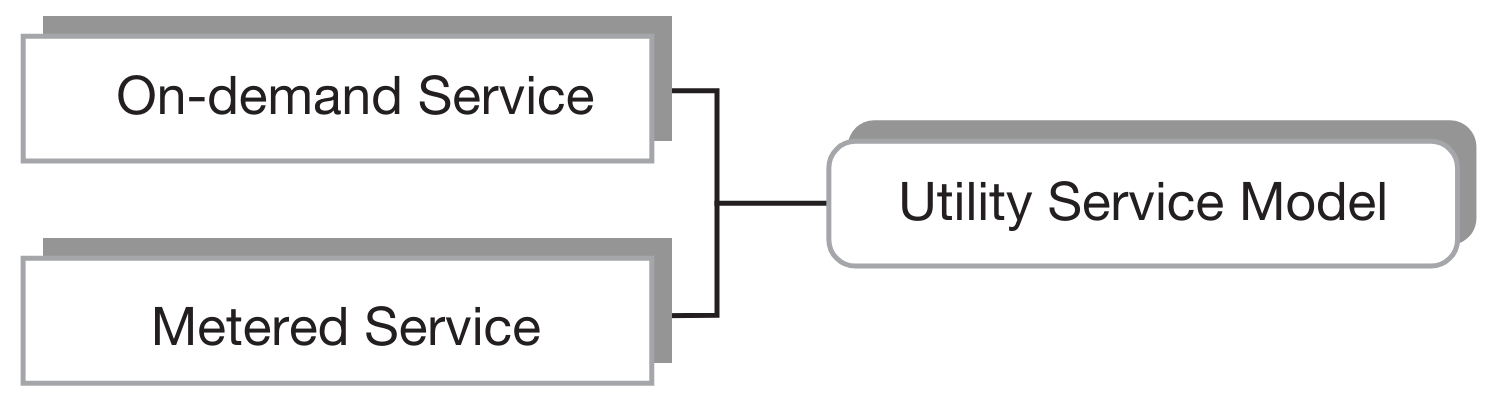
\includegraphics[width=0.5\textwidth]{image/fig 3.1.png}
                \caption{مدل سودمند ارائه خدمات}
                \label{fig:fig_3.1}
        
            \end{figure}

            در مدل کاربردی، تسهیلات محاسباتی به همراه منابع محاسباتی (شامل پردازنده، ذخیره‌سازی و غیره) به صورت بسته‌بندی شده ارائه می‌شود که می‌توان از محل دور دسترسی پیدا کرد. هزینه محاسباتی در این مدل محاسباتی کاهش می‌یابد زیرا همان مجموعه منابع بین تعداد زیادی از مشترکین به اشتراک گذاشته می‌شود. در اینجا، مشترکین می‌توانند با استفاده از مسیرهای ارتباطی شبکه‌ای یا شبکه‌های اینترنت، به تقریباً تامین ناپایانی از راه‌حل‌های محاسباتی دسترسی پیدا کنند.

            \begin{addinfo}
                
                تامین منابع توسط طرف ارائه‌دهنده بر اساس تقاضای کاربران به عنوان «خدمات درخواستی» شناخته می‌شود.

            \end{addinfo}

            ،IBM HP و Microsystems Sun در پایان قرن گذشته ابتکارات محاسباتی کاربردی خود را آغاز کردند. این شرکت‌ها سرمایه زیادی را برای انجام تحقیقات در مورد محاسبات درخواستی سرمایه‌گذاری کردند. آن‌ها رهبران در ابتکارهای توسعه محاسبات کاربردی بودند. بعدها، مایکروسافت، گوگل، آمازون و دیگران به این رقابت پیوستند.

            \subsection{مزایا}

                همانطور که در فصل ۱ بحث شده است، در اوایل قرن بیستم، ارائه برق به عنوان خدمات عمومی نگرانی‌ها و شکوفایی‌های مردم را برانگیخت. محاسبات به عنوان خدمات کاربردی نیز شبیه این نگرانی‌ها را به وجود می‌آورد. بحث‌ها در مورد مزایا و معایب برون‌سپاری محاسبات به عنوان خدمات کاربردی منظم است. دو گزینه در دسترس است؛ یا نگه‌داری مرکز داده خود، یا مصرف خدمات محاسبات ابری.

                برای برق بیش از یک قرن پیش، زمانی که برق به عنوان خدمات کاربردی در دسترس نبود، کسب‌وکارها باید تیم داخلی را نگه دارند یا کار نگه‌داری و اجرای نیروگاه‌های تولید برق را داخل ساختمان خود برون‌سپاری کنند. محاسبات در شکل سنتی خود به همان روش در مرکز داده خود سازمان حفظ می‌شود. اما چه اتفاقی می‌افتد زمانی که یک شرکت یا سازمان وظایف اجرای مرکز داده خود را به یک شخص ثالث برون‌سپاری می‌کند؟ یا چقدر مطلوب است که مرکز داده خود را با استفاده از تیم داخلی اجرا کند، زمانی که سازمان در زمینه محاسبات تخصص ندارد؟ در اینجا گزینه سوم وارد می‌شود. محاسبات ابری که تقریباً کلیه تسهیلات محاسباتی برون‌سپاری می‌شود اما به شکلی کاملاً متفاوت. سوال پیش می‌آید که آیا این گزینه ایمن‌تر از دو گزینه اولیه به شرکت‌های معتبری که در زمینه محاسبات تخصص دارند، مسئولیت‌ها را واگذار کنند. مدل کاربردی برون‌سپاری هزینه‌های عملیات فناوری اطلاعات را برای مشتریان به شکل قابل توجهی کاهش می‌دهد که یک مزیت بزرگ در این بازار بسیار چالشی است. محاسبات کاربردی همچنین مدل سرمایه‌گذاری را از سرمایه‌گذاری یکبار در سرمایه‌گذاری‌های کوچک و متغیر منتقل می‌کند.
            
                این نوع مدل محاسباتی نیز به ارائه‌دهندگان خدمات محاسباتی منافع می‌رساند. سرمایه‌گذاری‌های آن‌ها در ساختارهای سخت‌افزاری و نرم‌افزاری می‌تواند چندین راه‌حل را فراهم کند و به تعداد زیادی از کاربران خدمات ارائه دهد. این در نهایت منجر به بازگشت بهتر سرمایه گذاری می‌شود.

                \begin{addinfo}
                    
                    مدل خدمات کاربردی امکان سرمایه‌گذاری اولیه بسیار پایینی را فراهم می‌کند و همچنین صرفه‌جویی در هزینه کلی برای مشترکین.

                \end{addinfo}

        \section{اندازه‌گیری و صورتحساب در ابر}

            در محاسبات ابری، اندازه‌گیری واقعی خدمات محاسباتی ممکن شده است. در مدل‌های محاسبات خوشه‌ای قبلی، تعدادی از عملیات اندازه‌گیری ابتدایی وجود داشت، اما این عملیات کافی برای اندازه‌گیری استفاده واقعی از خدمات نبود. پیشرفت‌های فناوری ترکیبی که در محاسبات ابری به کار گرفته شده است، این قابلیت را فراهم می‌کند که مصرف توسط مشترکین با دقت اندازه‌گیری شود.

            استفاده‌ها برای انواع مختلف تسهیلات مانند پردازش، ذخیره‌سازی یا پهنای باند شبکه اندازه‌گیری می‌شوند. مشترکین بر اساس استفاده‌شان از منابع محاسباتی صورتحساب می‌گیرند. به عنوان مثال، یک مشترک که از تسهیلات محاسباتی در محاسبات ابری استفاده می‌کند، بر اساس استفاده از قدرت محاسباتی (هم پردازنده و هم حافظه)، استفاده از ذخیره‌سازی (در صورت وجود) و مصرف پهنای باند شبکه خود در طول زمان صورتحساب می‌شود. مشترکینی که از تسهیلات ذخیره‌سازی در ابر استفاده می‌کنند، بر اساس حجم ذخیره‌سازی واقعی مورد استفاده‌شان صورتحساب می‌شوند. قابلیت اندازه‌گیری محاسباتی ابری منجر به صرفه‌جویی قابل توجهی در هزینه برای کاربران می‌شود.

            \begin{addinfo}
                
                در محاسبات سنتی، عملیات اندازه‌گیری ابتدایی کافی برای اندازه‌گیری استفاده واقعی از محاسبات نبود. اما محاسبات ابری با این توانایی مجهز شده است.

            \end{addinfo}

        \section{جداسازی عملیات مرکز داده}

            عملیات مرکز داده محاسباتی همواره برای بیشتر مصرف کنندگان محاسبات، به ویژه شرکت‌ها، بار سنگینی بوده است. عملیات مرکز داده شامل تنظیم فضا برای توسعه زیرساخت، اطمینان از تأمین برق بدون وقفه، ایجاد سیستم خنک‌کننده و به‌ویژه ساخت زیرساخت محاسباتی و غیره می‌شود. علاوه بر این‌ها، نگهداری سیستم، اجرای به‌روزرسانی‌ها، بازیابی در صورت خرابی سیستم یا حفاظت از سیستم در برابر حملات شبکه، همه فعالیت‌های انتهای مرکز داده هستند. مدل محاسبات ابری کاملاً عملیات مرکز داده را از وظایف محاسباتی کاربر پایانی (مانند توسعه برنامه) جدا می‌کند. توسعه دهندگان نرم‌افزار یا کاربران برنامه همیشه سعی کرده‌اند از وظایف مدیریت زیرساخت محاسباتی خود دوری کنند. بنابراین، در مدل محاسبات سنتی، برون‌سپاری مدیریت مرکز داده ویژگی متداولی بوده است.

            در محاسبات ابری، مراکز داده در یک انتهای دور اقامت دارند و توسط چند فروشنده محاسبات مدیریت می‌شوند. فروشنده همه چیز را تنظیم و مدیریت می‌کند. کاربران می‌توانند به طور کامل و کاملاً تمرکز خود را بر روی وظایف خاص خود متمرکز کنند. این امکان به عنوان یک تسکن بزرگ برای کاربران محاسباتی آمده است.

            \begin{addinfo}
                
                محاسبات ابری عملیات مرکز داده را از سایر فعالیت‌ها در انتهای کاربران جدا می‌کند.

            \end{addinfo}

        \section{مزایای رایانش ابری}

            محاسبات ابری یک تغییر دیگر در دامنه محاسبات را به وجود آورده است. برخلاف استفاده‌های معمول فناوری کامپیوتر، این امکان را فراهم می‌کند که محاسبات به عنوان یک خدمات کاربردی ارائه شود که بر اساس درخواست ارائه می‌شود. تسهیلات محاسباتی توسط ارائه‌دهندگان مدیریت می‌شود و می‌تواند به حجم استفاده یا زمان استفاده اندازه‌گیری شود.

            همه این ویژگی‌های محاسبات ابری چندین مزیت ارائه می‌دهد. این امکان را دارد که کاربران در هر زمان دلخواهشان به اندازه‌ی خودشان بخواهند استفاده کنند. این مزایا تأثیر گذاری بر انتخاب محاسبات ابری را نسبت به روش محاسباتی سنتی دارد. بخش بعدی به مزایای مختلفی که مشترکان محاسبات ابری می‌توانند بهره‌مند شوند، می‌پردازد.

            \subsection{هزینه اکتساب / خرید کمتر}

                در محاسبات سنتی، کاربران باید منابع محاسباتی را به میزان قابل توجهی در ابتدا خریداری یا تهیه کنند. محاسبات ابری طبق مدل خدمات کاربردی ارائه می‌شود. از آنجایی که فروشنده در این مدل تمام منابع مورد نیاز را تنظیم می‌کند، سرمایه‌گذاری اولیه مشترکان برای تهیه سخت‌افزار یا نرم‌افزار به طور چشمگیری کاهش می‌یابد. آنها نیازی به تنظیم هیچ چیزی جز سیستم‌های مشتری برای دسترسی به خدمات ابری ندارند. بنابراین، هزینه سرمایه‌گذاری اولیه کاربر به طور قابل توجهی کاهش می‌یابد.

                \begin{addinfo}
                    
                    سرمایه‌گذاری اولیه کاربرانی که به محاسبات ابری می‌پردازند، بسیار کم است.

                \end{addinfo}

            \subsection{کاهش هزینه عملیاتی}

                با مدل برون‌سپاری محاسبات کاربردی، هزینه اجرای هر سیستم به صورت ۲۴ ساعته به سمت ارائه‌دهنده متمایل می‌شود. مشترکان از مسئولیت مدیریت سیستم، نگهداری و پشتیبانی انرژی ۲۴ × ۷ و همچنین پشتیبانی از خنک‌کننده خلاص می‌شوند. این اساس صرفه‌جویی در هزینه است زیرا مشترکان می‌توانند خدمات را با پرداخت مبلغ بسیار کم استفاده کنند. از طرف دیگر، ارائه‌دهنده می‌تواند خدمات را با هزینه کم به مشترکان ارائه دهد به دلیل حجم کسب و کار خود (به دلیل وجود پایگاه مشتریان بزرگ).

                \begin{addinfo}
                    
                    مشترکان خدمات محاسبات ابری باید هزینه عملیاتی ناچیزی را تحمل کنند.

                \end{addinfo}

            \subsection{کاهش مسئولیت مدیریت سیستم}

                باشد مرکز داده برای شرکت‌ها یا یک دستگاه مستقل (کامپیوتر شخصی، لپ‌تاپ و غیره) برای کاربران عادی، مدیریت تنظیمات محاسباتی (هم سخت‌افزار و هم نرم‌افزار) برای مصرف‌کنندگان محاسبات سنتی یک سرگرمی اضافی است. مدل محاسبات ابری اکثر تسهیلات زیرساختی و سایر وظایف مدیریت سیستم را به سمت فروشندگان ابری منتقل می‌کند. تیم‌های اختصاصی در انتهای فروشنده از تمام این فعالیت‌ها مراقبت می‌کنند. بنابراین، کاربران می‌توانند احساس آسایش کنند و تنها بر روی حوزه (لایه) خاص محاسباتی خود تمرکز کنند بدون این که نگران مدیریت لایه‌های زیرین محاسباتی باشند.

                \begin{addinfo}
                    
                    محاسبات ابری باعث آزادی کاربران از وظیفه مدیریت سیستم محاسباتی زیرین می‌شود.

                \end{addinfo}
                

    %%%%%%%%%%%%%%%%%%%%%%%%%%%%%%%%%%%%%%%%%%%%%%%%%%%%%%%%%%%%%%%%%%%%%%%%%%%%%%%%%%%%%%%%%%%%%%%%
    %%%%%%%       Shara        %%%%%%%%%%%%%%%%%%%%%%%%%%%%%%%%%%%%%%%%%%%%%%%%%%%%%%%%%%%%%%%%%%%%%
    %%%%%%%%%%%%%%%%%%%%%%%%%%%%%%%%%%%%%%%%%%%%%%%%%%%%%%%%%%%%%%%%%%%%%%%%%%%%%%%%%%%%%%%%%%%%%%%%

    \subsection{امکان پرداخت بر اساس استفاده}

        محاسبات ابری هزینه‌ای را برای مشترکانشان در زمانی که از آن استفاده نمی‌شوند، دریافت نمی‌کنند. حتی هزینه‌ی آن ثابت نیست؛ بلکه بستگی به مدت استفاده دارد. به جای آن، هر استفاده‌ای اندازه‌گیری می‌شود و کاربران بر اساس مصرف خود، هزینه‌ی مناسبی پرداخت می‌کنند. این باعث کاهش هزینه‌های محاسباتی می‌شود.

    \subsection{قدرت محاسباتی و ذخیره‌سازی نامحدود}

        در محاسبات ابری، کاربران می‌توانند به طور آسان به قدرت محاسباتی شبیه به یک سوپرکامپیوتر با هزینه‌ای مناسب دسترسی پیدا کنند، در صورت نیاز. در روش سنتی، تنها شرکت‌های بزرگ می‌توانستند هزینه‌های کامپیوتری پیشرفته را تحمل کنند. ذخیره‌سازی نیز یک مسئله مهم برای کاربران است. ابر به اندازه‌ای ذخیره‌سازی فراهم می‌کند که لازم است. این تقریباً نامحدود است که به عنوان یک مزیت بزرگ برای کاربران می‌تواند مشاهده شود.

    \subsection{کیفیت خدمات}

        در محاسبات سنتی، شرکت‌ها اغلب بخش‌های اصلی از کارهای مرتبط با محاسبات را به شرکای سومی برون‌سپاری می‌کردند. بنابراین، کیفیت خدمات به طور گسترده از تخصص شرکای سوم یا تیم‌های داخلی مدیریت آن وابسته بود. در حالی که در محاسبات ابری، کیفیت بالای خدمات (QoS) تضمین می‌شود زیرا توسط تامین‌کنندگان معتبر محاسباتی که دارای کارکنان آموزش‌دیده و تخصص دارند، ارائه می‌شود که به طور اختصاصی در زمینه محاسبات فعالیت می‌کنند.
    
    \begin{addinfo}
        
        وقتی خدمات توسط تامین‌کنندگان معروف ارائه می‌شود، کیفیت خدمات تضمین می‌شود و این وظیفه تامین‌کننده می‌شود.

    \end{addinfo}

    \subsection{اعتماد‌پذیری}

        توانایی ارائه خدمات با کیفیت و پشتیبانی از توازن بار، پشتیبان‌گیری و بازیابی در صورت عدم موفقیت، باعث می‌شود که تامین‌کنندگان ابر معروف بسیار قابل اعتماد باشند که اغلب به عنوان یک مشکل بزرگ در محاسبات سنتی مطرح می‌شود. در محاسبات ابری، مشترکان دیگر نیازی به برنامه‌ریزی برای همه این وظایف پیچیده ندارند زیرا تامین‌کنندگان این مسائل را در دست می‌گیرند و آنها را بهتر انجام می‌دهند.

    \subsection{پیوستگی در دسترسی}

        تامین‌کنندگان معتبر ابر تقریباً اطمینان از دسترسی به خدمات 24 ساعته و 7 روزه را فراهم می‌کنند. آمار نشان داده است که زمان فعالیت سرویس (ارائه شده توسط تامین‌کنندگان معتبر) در طول یک سال معمولاً به کمتر از 99.9٪ نمی‌رسد. این پایداری مداوم تضمین‌شده خدمات ابر برای هر کسب و کاری یک مزیت بزرگ است.

    \subsection{استقلال مکانی/راحتی دسترسی}

        محاسبات ابری از طریق اینترنت در همه جا در دسترس است. کاربران می‌توانند از طریق هر دستگاه محاسباتی مانند کامپیوترهای شخصی یا دستگاه‌های قابل حمل مانند تبلت، لپ‌تاپ یا تلفن هوشمند به آن دسترسی پیدا کنند. تنها چیزی که برای بهره‌مندی از محاسبات ابری از طریق این دستگاه‌ها لازم است، دسترسی به اینترنت است، بدون توجه به مکان جغرافیایی یا منطقه زمانی.

    \begin{addinfo}

        راحتی دسترسی و سرمایه‌گذاری کم، محاسبات ابری را به یک حوزه با حداقل مانع ورود تبدیل کرده‌است.

    \end{addinfo}

    \subsection{مقاومت بالا}

        مقاومت توانایی کاهش شدت و/یا مدت مختل شدن توسط شرایط ناخواسته است. سطح بالاتری از مقاومت ارزش بسیاری در محیط محاسباتی دارد. محاسبات ابری بر پایه زیرساخت محاسبات مقاوم ساخته شده‌است و بنابراین خدمات ابری به حملات و اشکالات بیشتری مقاومت دارند. مقاومت زیرساختی از طریق تکرار زیرساخت همراه با مکانیزم مؤثری برای پیش‌بینی، جذب و سازگاری دست‌یافته می‌شود. مصرف‌کنندگان ابر می‌توانند با بهره‌گیری از مقاومت منابع IT مبتنی بر ابر، اعتبار کسب‌وکارهای خود را افزایش دهند.

    \subsection{راه‌اندازی سریع}

        زمان راه‌اندازی در محیط ابر به طرز قابل توجهی کاهش یافته است نسبت به آنچه در محیط محاسبات سنتی بود. این امکان از طریق تأمین منابع سریع و خودکار در محیط ابر فراهم می‌شود. در یک بازار بسیار رقابتی، توانایی راه‌اندازی سریع مزایای کسب و کار قابل توجهی را به دنبال دارد.

    \begin{addinfo}

        راه‌اندازی سریع‌تر سیستم یا برنامه مزیت تجاری را در بازار رقابتی به دست می‌آورد.

    \end{addinfo}

    \subsection{به‌روزرسانی‌های نرم‌افزاری خودکار}

        مسئله به‌روزرسانی نرم‌افزار در محیط محاسبات سنتی بسیار زحمت‌آور است. به‌طور دوره‌ای پچ‌های جدید منتشر می‌شوند و کاربران باید این پچ‌ها را به طور دوره‌ای اجرا کنند. در محیط محاسبات ابری، این به‌روزرسانی به‌صورت خودکار اتفاق می‌افتد. تامین‌کنندگان ابر همواره آخرین نسخه موجود هر نرم‌افزار را (مگر اینکه درخواست دیگری داده شده باشد) ارائه می‌دهند. محیط به‌روزرسانی‌شده تقریباً فوراً پس از ارائه در دسترس کاربران قرار می‌گیرد، و هر زمان کاربر بعدی وارد سیستم شود، موجود خواهد بود.

    \subsection{تهیه مجوز نیاز نیست}

        تهیه مجوز برنامه‌ها نیازمند ترتیبات بودجه‌ای جداگانه در محاسبات سنتی بود. علاوه بر این، برنامه‌های اضافی معمولاً با بسته‌های مجوزی ارائه می‌شدند. محاسبات ابری نیز این مشکل را برطرف کرده است. در اینجا، کاربران نیازی به تهیه هرگونه مجوز دوره‌ای برای استفاده از برنامه‌ها ندارند؛ بلکه به آنها اجازه می‌دهند که بر اساس استفاده‌شان از هر نرم‌افزار، پرداخت کنند (پس از پرداخت).
    
    \begin{addinfo}

        در محاسبات ابری، مجوز نرم‌افزار دیگر نگرانی برای کاربران نیست.

    \end{addinfo}

    \subsection{امنیت در برابر فاجعه}

        خرابی سیستم به دلیل شکست فنی ناگهانی یا فاجعه طبیعی نگرانی اصلی برای کاربران است. به ویژه، هرگونه آسیب به دستگاه‌های ذخیره‌سازی فیزیکی ممکن است باعث ضرر تجاری عظیم شود. محاسبات ابری ارائه شده توسط تامین‌کنندگان معتبر دارای سیستم‌های بازیابی قدرتمندی در تنظیمات خود است. بنابراین، سیستم‌ها و داده‌ها از لحاظ ایمنی و امنیت، در محاسبات ابری نسبت به سیستم‌های قبلی بیشتر محافظت می‌شوند.

    \subsection{دوستی به محیط زیست}

        محاسبات ابری از محیط زیست دوستانه حمایت می‌کند. استفاده مناسب از منابع، نیاز کلی به منابع الکترونیکی را کاهش می‌دهد، بنابراین تولید زباله‌های الکترونیکی را نیز کاهش می‌دهد. این برای محیط زیست مفید است زیرا اگر زباله‌های الکترونیکی به درستی پردازش نشوند، برای اکوسیستم مضر هستند. علاوه بر این، کاهش نیاز به منابع منجر به کاهش تقاضا و بنابراین تولید منابع محاسباتی می‌شود. این کاهش در تولید الکترونیکی باعث کاهش انتشار کربن و کمک به کاهش کلی ردپای کربن می‌شود.

    \begin{addinfo}
        
        محاسبات ابری یک رویکرد محاسباتی سبز و دوستدار محیط زیست است.

    \end{addinfo}

        این لیست طولانی از مزایایی که در بالا بحث شد، در شکل ۳.۲ نمایش داده شده‌اند. آنها نشان می‌دهند که محاسبات ابری چه قدر مفید است و چرا انقدر افراد به آن مشتاق هستند.

    \begin{figure}[htbp]

        \centering
        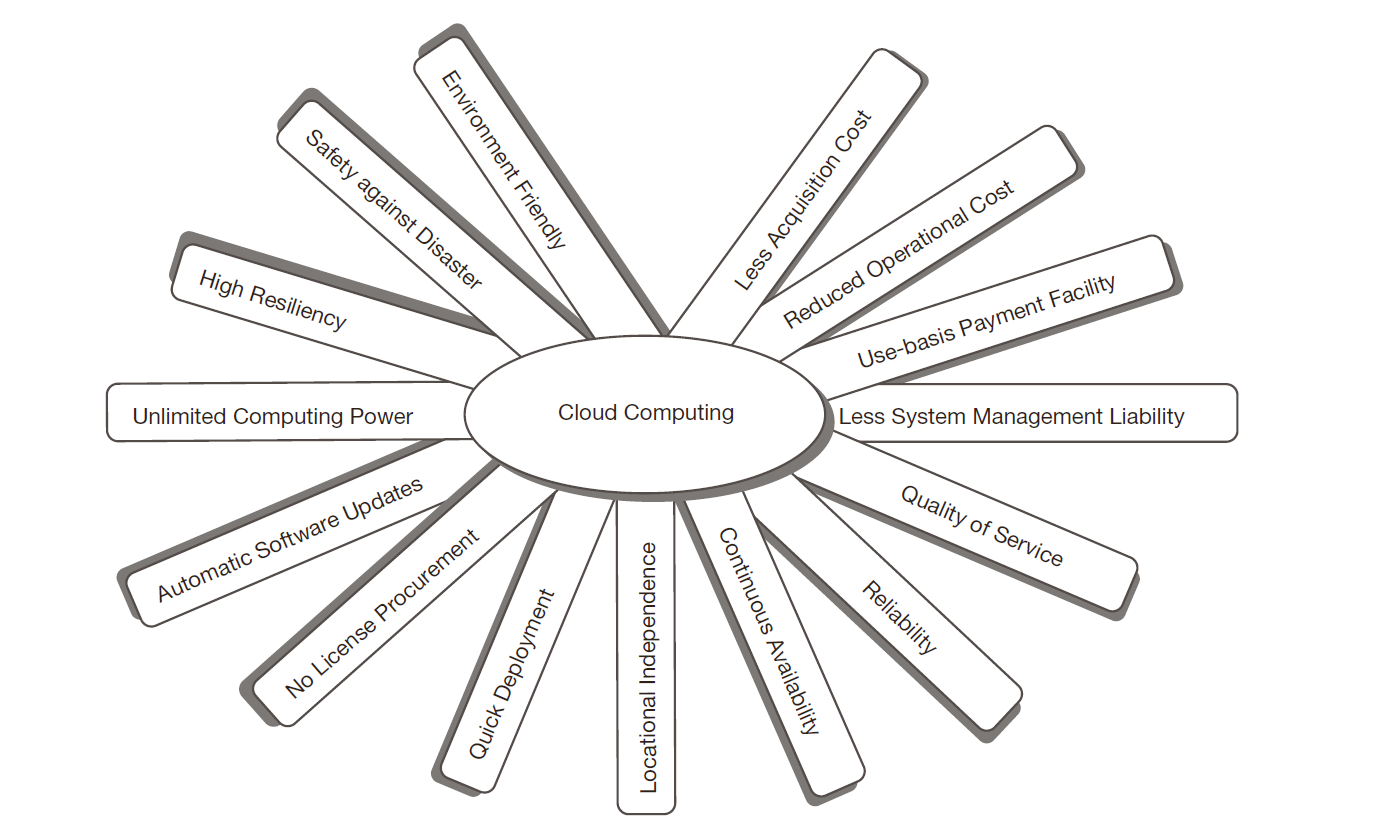
\includegraphics[width=1\textwidth]{image/fig 3.2.png}
        \caption{مزایای محاسبات ابری}
        \label{fig:fig_3.2}

    \end{figure}

    \section{چالش‌های محاسبات ابری}

        محاسبات ابری بهره‌های فراوانی ارائه می‌دهد. اما، مانند هر فناوری جدیدی، این مدل محاسباتی هم چالش‌های خود را به همراه دارد. بخش زیر بر روی این چالش‌ها تمرکز می‌کند. قسمت خوب این است که تمامی ارگان‌های مرتبط، شامل تامین‌کنندگان ابری، به دقت برای غلبه بر این چالش‌ها کار می‌کنند.
    
    \subsection{محدودیت‌های قابلیت‌حملی بین ارائه‌دهندگان ابر}

        محاسبات ابری در دوران اولیه خود قرار دارد و یک استانداردکاری کلی هنوز در این حوزه مطرح نشده است. به طبیعت کار، ارائه‌دهندگان مختلف ابری امکانات محاسبات ابری را برای استفاده عمومی ارائه می‌دهند که بیشتر به اندازه‌های مختلف به صورت مختصات است. برنامه‌های توسعه‌یافته بر روی این ابرهای مختصات به دلیل قفل شدن توسط تامین‌کننده، دشواری در انتقال به پلتفرم‌های ابری دیگر دارند. این مشکل قابلیت‌حملی برنامه‌ها را محدود می‌کند. بنابراین، بسیاری اوقات انتقال از یک ارائه‌دهنده ابر به دیگری چالشی است. تلاش‌های مختلفی برای حل این مسئله در حال انجام است.

    \begin{addinfo}

        در حال حاضر، مشکل قفل شدن توسط تامین‌کننده، قابلیت‌حمل برنامه‌های ابری را محدود می‌کند.

    \end{addinfo}

    \subsection{مشکل تعامل‌پذیری}

        تعامل‌پذیری، توانایی یک سیستم برای کار با سیستم‌های دیگر است. مسئله مخصوصیت مورد بحث بالا، نه تنها مشکل قابلیت‌حمل را افزایش می‌دهد، بلکه همچنین محدودیت‌هایی را در تعامل بین دو برنامه از دو ابر مختلف به وجود می‌آورد. این به عنوان مسئله تعامل‌پذیری شناخته می‌شود. برنامه‌های دو ابر مختلف مخصوصیت اجرایی را دنبال می‌کنند و به همین دلیل همگام نمی‌شوند. مشترکین ممکن است دو برنامه متفاوت از دو تامین‌کننده ابر مختلف را برای نیازهای خود مناسب ببینند. به عنوان مثال، یک شرکت ممکن است برنامه مدیریت حقوق و دستمزد یک تامین‌کننده ابر را دوست داشته باشد در حالی که برنامه مدیریت حساب‌ها را از تامین‌کننده دیگر. اما اگر این دو برنامه تعامل‌پذیر نباشند، برقرار کردن ارتباط بین آنها دشوار است. تلاش‌هایی برای حل این مسئله انجام شده است. توسعه برنامه با استفاده از استانداردهای باز (همانند آنچه بعداً بحث خواهد شد) یک گام در این راستا است.

    \begin{addinfo}
        
        استفاده از فناوری‌های مخصوص، محدودیت‌هایی را برای تعامل بین برنامه‌های دو تامین‌کننده ابر مختلف به وجود می‌آورد.

    \end{addinfo}

    \subsection{امنیت داده}

        در محاسبات ابری، کاربران یا شرکت‌ها نیاز دارند که داده‌های خود را خارج از محدوده شبکه‌ی خود که توسط دیواره‌های آتشین محافظت می‌شود، ذخیره کنند. بنابراین، مرز اعتماد شرکت‌ها تا ابر خارجی گسترش می‌یابد. امنیت داده‌های کاربران بیشتر به تامین‌کنندگان ابر وابسته است. این ممکن است موجب بروز نقاط ضعفی در امنیت داده‌ها شود. یک مشکل دیگر پیش می‌آید زمانی که یک امکان محاسبات ابری که توسط چندین نهاد دسترسی دارد، باعث اشتراک مرز اعتماد میان موارد مختلف شود.
    
    \begin{addinfo}

        ایجاد اعتماد در میان مصرف‌کنندگان در مورد امنیت داده‌های کاربر/شرکتی که خارج از مرز شبکه خود ذخیره می‌شود، یک چالش بزرگ در محاسبات ابری است.
        
    \end{addinfo}

    \subsection{کاهش کنترل بر مدیریت}

        در محاسبات ابری، ساختار و حکومت توسط سیاست‌های تامین‌کننده محاسبات یا ارائه‌دهنده خدمات تعیین می‌شود. مصرف‌کنندگان از مسئولیت خسته‌کننده مدیریت سیستم محاسباتی آزاد شده‌اند. اگرچه این به عنوان یک مزیت اساسی در نظر گرفته می‌شود، اما کاهش کنترل بر مدیریت یا اختیار محیط محاسباتی گاهی نگرانی‌ها را در میان مصرف‌کنندگان ایجاد می‌کند که قبلاً از کنترل کامل بر مراکز داده سنتی خود لذت می‌بردند. اصلی‌ترین نگرانی مربوط به نحوه عملکرد یک تامین‌کننده ابر است. اگرچه کنترل عملیاتی کمی به مشترکین داده می‌شود اما بسته به نوع خدمت و توافقنامه سطح خدمات نقش مهمی در این زمینه ایفا می‌کند.

    \begin{addinfo}
        
        کاهش کنترل بر مدیریت ابر ممکن است گاهی اوقات مشترکان محاسبات ابری را نگران کند.
        
    \end{addinfo}

    \subsection{مسائل قانونی و اطمینان از تطابق چندمنطقه‌ای}

        تامین‌کنندگان محاسبات ابری دیتاسنترها را در مکان‌هایی که برایشان مناسب است، هم از نظر جغرافیایی و هم از نظر اقتصادی، ایجاد می‌کنند. یک تامین‌کننده ممکن است حتی بیش از یک دیتاسنتر را در مکان‌های جغرافیایی مختلف داشته باشد. از آنجا که مشترکین به طور دور از طریق اینترنت به محاسبات ابری دسترسی پیدا می‌کنند، ممکن است از مکان واقعی منابعی که مصرف می‌کنند آگاه نباشند. به طور مهمی‌تر، مکان ذخیره‌سازی داده‌های مشترک ممکن است در داخل کشور یا منطقه مشترک قرار نگیرد. این گاهی نگرانی‌های قانونی جدی را به وجود می‌آورد.

        قوانین حفظ حریم خصوصی یا اطمینان از تطابق به طور عمومی در اقلیت‌های قانونی مختلف متفاوت است. قوانین برای درجه افشای داده‌های شخصی به ادارات دولتی (در صورت بررسی‌های رسمی) از کشور به کشور متفاوت است، یا حتی از ایالت به ایالت درون یک کشور متفاوت است. ممکن است موقعیتی پیش آید که قانون کشور یک مشترک ابری بخواهد برخی از داده‌ها را افشا کند در حالی که قانون منطقه میزبان ابر (یعنی منطقه/کشور دیتاسنتر ابر) چنین افشایی را مجاز نمی‌کند.

        بیشتر چارچوب‌های قوانینی، سازمان‌های مصرف‌کننده ابر را مسئول امنیت، صحت و ذخیره‌سازی داده‌ها حتی زمانی که در واقع توسط تامین‌کننده‌های ابر خارجی نگهداری می‌شوند، تشخیص می‌دهند. در چنین وضعیتی، حل مسائل قانونی و اطمینان از تطابق چندمنطقه‌ای چالش‌های بزرگی برای محاسبات ابری می‌باشد.
    
    \begin{addinfo}
        
        مسائل قانونی چندمنطقه‌ای نگرانی‌ها درباره حریم خصوصی اطلاعات و مشکلات مربوط به اطمینان از تطابق در محاسبات ابری را افزایش می‌دهد.
        
    \end{addinfo}

    \subsection{هزینه پهنای باند}

        این یک چالش به اندازه‌ی چالش‌های دیگر مطرح شده بالا مهم نیست. اما واقعیت این است که در حالی که مدل پرداخت براساس استفاده از محاسبات ابری هزینه‌ها را کاهش می‌دهد چرا که مشترکین تنها برای منابع یا خدماتی که استفاده می‌کنند پرداخت می‌کنند، اما این مدل هزینه‌های مرتبطی را به همراه دارد. هزینه پهنای باند شبکه که برای دسترسی به خدمات استفاده می‌شود از جمله آنهاست.

        در عصر فعلی اینترنت، هزینه پهنای باند به سرعت متوسط دسترسی بسیار پایین است. اما بیشتر پهنای باند می‌تواند سرعت بالاتری را فراهم کند که برای ارائه خدمات با کیفیت بالا ضروری است. در حالی که پهنای باند با هزینه کم معمولاً نیازهای برنامه‌های عمومی را برآورده می‌کند، برنامه‌های داده‌محور (که با مجموعه داده‌های بحرانی و حجیم سر و کار دارند) نیاز به پهنای باند بیشتری دارند که ممکن است هزینه کل محاسبات را کمی بیشتر کند.

        \begin{addinfo}
            
            هزینه پهنای باند شبکه یک هزینه اضافی در محاسبات ابری است.
            
        \end{addinfo}
        
\end{document}